\documentclass[12pt,a4paper]{article}
\newif\ifchronologia
\ifdefined\Chronologia\chronologiatrue\else\chronologiafalse\fi
\usepackage[utf8]{inputenc}
\usepackage[OT4,plmath]{polski}
\usepackage{amsmath,amssymb,amsthm}
\usepackage[a4paper,margin=27mm]{geometry}
\usepackage{microtype}
\usepackage{graphicx}
\usepackage{eso-pic}
\usepackage[hidelinks,unicode]{hyperref}

\hypersetup{pdftitle={Nieliniowa Analiza Funkcjonalna}}
\setlength{\parindent}{1.5em}
\setlength{\parskip}{0pt}
\allowdisplaybreaks[1]
\theoremstyle{definition}
\newtheorem{definicja}{Definicja}
\newtheorem{przyklad}{Przykład}
\newtheorem{uwaga}{Uwaga}
\theoremstyle{plain}
\newtheorem{fakt}{Fakt}
\newtheorem*{faktbeznum}{Fakt}
\newtheorem{twierdzenie}{Twierdzenie}
\newtheorem{lemat}{Lemat}
\newtheorem{wniosek}{Wniosek}
\renewcommand{\proofname}{Dowód}
\newcommand{\R}{\mathbb{R}}
\newcommand{\C}{\mathbb{C}}
\newcommand{\N}{\mathbb{N}}
\newcommand{\Z}{\mathbb{Z}}

% Znaczniki wykładów nie zmieniają treści ani numeracji matematycznej.
\newcommand{\poczatekwykladu}[1]{%
  \ifchronologia
    \par\addvspace{\baselineskip}%
    \phantomsection
    \addcontentsline{toc}{section}{Wykład #1}%
    \noindent{\large\bfseries Wykład #1}\par\nobreak
    \noindent\rule{\linewidth}{0.4pt}\par\nobreak
    \addvspace{0.5\baselineskip}%
  \fi
}

\begin{document}

% Okładka wypełnia całą pierwszą stronę A4.
\hypersetup{pageanchor=false}
\begin{titlepage}
  \thispagestyle{empty}
  \AddToShipoutPictureBG*{%
    \AtPageLowerLeft{%
      
\includegraphics[width=\paperwidth,height=\paperheight]{../grafika/okladka.png}%
    }%
  }
  \null
\end{titlepage}
\hypersetup{pageanchor=true}
\pagenumbering{arabic}
\pagestyle{plain}

\poczatekwykladu{1}
\section{Wstęp}

Zajmujemy się narzędziem opisującym liczbę rozwiązań równania $f(x) = y$ w przestrzeni rzeczywistej skończenie wymiarowej.
W tym celu kładziemy funkcję:
\[
d\colon
\left\{
  (f,\Omega,y)\;\middle|\;
  \begin{array}{l}
    \Omega\subset\R^n\text{ jest otwarty i ograniczony},\\
    f\colon\overline{\Omega}\to\R^n\text{ jest ciągła},\\
    y\in\R^n\setminus f(\partial\Omega)
  \end{array}
\right\}
\longrightarrow\Z,
\]
spełniającą następujące własności:

\begin{enumerate}
  \item[(d1)] \textbf{Normalizacja.} Dla $y\in\Omega$ zachodzi
  \[
    d(\operatorname{id},\Omega,y)=1.
  \]

  \item[(d2)] \textbf{Addytywność.} Jeżeli $\Omega_1,\Omega_2\subset\Omega$
  są rozłącznymi zbiorami otwartymi oraz
  \[
    y\notin f\bigl(\overline{\Omega}\setminus(\Omega_1\cup\Omega_2)\bigr),
  \]
  to
  \[
    d(f,\Omega,y)=d(f,\Omega_1,y)+d(f,\Omega_2,y).
  \]

  \item[(d3)] \textbf{Niezmienniczość homotopijna.} Niech $J=[0,1]$.
  Jeżeli odwzorowania
  \[
    h\colon J\times\overline{\Omega}\to\R^n,
    \qquad y\colon J\to\R^n
  \]
  są ciągłe i dla każdego $t\in J$ spełniają warunek
  \[
    y(t)\notin h(t,\partial\Omega),
  \]
  to liczba
  \[
    d\bigl(h(t,\cdot),\Omega,y(t)\bigr)
  \]
  jest niezależna od $t\in J$.
\end{enumerate}

Nazywamy ją \textbf{stopniem topologicznym równania $f(x) = y$ na zbiorze $\Omega$}.

\begin{uwaga}
$(d3)$ oznacza tyle, że wewnątrz $\Omega$ rozwiązania mogą się przesuwać, powstawać albo znikać, jednak ich łączny wkład do stopnia topologicznego pozostaje taki sam.
\end{uwaga}

\section{Jednoznaczność stopnia}

Przed podaniem wzoru na stopień topologiczny chcemy wykazać, że:

\begin{twierdzenie}
\label{tw:jednoznacznosc-stopnia}
Istnieje co najwyżej jedna funkcja
\[
d\colon
\left\{
  (f,\Omega,y)\;\middle|\;
  \begin{array}{l}
    \Omega\subset\R^n\text{ jest otwarty i ograniczony},\\
    f\colon\overline{\Omega}\to\R^n\text{ jest ciągła},\\
    y\in\R^n\setminus f(\partial\Omega)
  \end{array}
\right\}
\longrightarrow\Z
\]
spełniająca własności (d1)--(d3).
\end{twierdzenie}

Dowód jest długi, więc dzielimy jego szkic na części.

\medskip

Określiliśmy $d$ dla trójek $(f,\Omega,y)$, w których funkcja $f$ jest ciągła
na domknięciu dziedziny $\Omega$. Z własności (d3) nasuwa się jednak myśl,
że wystarczy analizować funkcje gładkie określone na całej przestrzeni.

Możemy przedłużyć funkcję na całą przestrzeń, ponieważ $d$ dalej zależy tylko
od jej wartości na $\overline{\Omega}$. Wygładzenie też jest legalne, jeśli
przybliżenie jest na tyle bliskie jednostajnie, że odpowiednia homotopia
nie wprowadza rozwiązań na brzegu. Pokażemy więc, jak funkcję ciągłą
przybliżać jednostajnie funkcjami gładkimi.

\medskip

\poczatekwykladu{2}
\begin{lemat}
\label{lem:przedluzenie-funkcji}
Jeżeli $A\subset\R^n$ jest zwarty, a $f\colon A\to\R^n$ jest ciągła,
to istnieje ciągła funkcja $\widetilde{f}\colon\R^n\to\R^n$ spełniająca
\[
  \left.\widetilde{f}\right|_A=f.
\]
\end{lemat}

\begin{proof}
Jeśli $A=\varnothing$, wystarczy przyjąć $\widetilde{f}\equiv0$.
Dla niepustego $A$ wybierzmy co najwyżej przeliczalny zbiór gęsty
$\{a_1,a_2,\ldots\}\subset A$. Przy zbiorze skończonym można powtarzać
jego punkty. Dla $x\notin A$ oznaczmy
\[
  \rho(x,A)=\inf_{a\in A}|x-a|>0,
  \qquad
  \varphi_j(x)=\max\left\{2-\frac{|x-a_j|}{\rho(x,A)},0\right\}.
\]
Definiujemy
\[
  \widetilde{f}(x)=
  \begin{cases}
    f(x), & x\in A,\\[2mm]
    \displaystyle
    \frac{\sum_{j=1}^{\infty}2^{-j}\varphi_j(x)f(a_j)}
         {\sum_{j=1}^{\infty}2^{-j}\varphi_j(x)}, & x\notin A.
  \end{cases}
\]

\begin{uwaga}
Oba szeregi we wzorze na $\widetilde{f}$ zbiegają jednostajnie na $A^c$.
Istotnie, $f$ jest ciągła na zbiorze zwartym $A$, więc
$K=\max_{a\in A}|f(a)|<\infty$. Dla każdego $z\in A^c$ mamy
\[
  0\leq 2^{-j}\varphi_j(z)\leq 2^{1-j},
  \qquad
  \bigl|2^{-j}\varphi_j(z)f(a_j)\bigr|\leq 2^{1-j}K.
\]
Szeregi liczbowe $\sum_{j=1}^{\infty}2^{1-j}$ i
$\sum_{j=1}^{\infty}2^{1-j}K$ są zbieżne. Z kryterium Weierstrassa
otrzymujemy więc jednostajną zbieżność obu szeregów funkcji.

Składniki obu szeregów są ciągłe na $A^c$. Funkcja odległości jest ciągła
i dodatnia na $A^c$, więc iloraz $|z-a_j|/\rho(z,A)$ jest ciągły.
Maksimum funkcji ciągłej i zera jest ciągłe, zatem każda $\varphi_j$ jest
ciągła na $A^c$. Mnożenie przez stałe $2^{-j}$ i $f(a_j)$ zachowuje ciągłość.
\end{uwaga}

\medskip
Chcemy wykazać, że $\widetilde{f}$ jest ciągła. Ustalmy $x_0\in\R^n$.

\begin{enumerate}
  \item[$1^\circ$] \textbf{Niech $x_0\notin A$.}

  \[
    \lim_{x\to x_0}\widetilde{f}(x)=\widetilde{f}(x_0).
  \]
  Zwartość $A$ pozwala odgrodzić $x_0$ kulą rozłączną z $A$.
  Granicę wprowadzamy do licznika i mianownika, a następnie pod oba szeregi,
  ponieważ są one jednostajnie zbieżne, a wszystkie $\varphi_j$ są ciągłe na $A^c$.

  \item[$2^\circ$] \textbf{Niech $x_0\in A$.}

  Wtedy $\widetilde{f}(x_0)=f(x_0)$. Ustalmy $\varepsilon>0$.
  Z ciągłości $f$ wybieramy $\delta_1>0$ takie, że
  \[
    a\in A,\quad |a-x_0|<\delta_1
    \quad\Longrightarrow\quad
    |f(a)-f(x_0)|<\varepsilon.
  \]

  Rozważmy najpierw $x\notin A$ spełniające
  \[
    |x-x_0|<\frac{\delta_1}{3}.
  \]
  Oznaczmy
  \[
    I(x)=\{j\geq1:\varphi_j(x)>0\}.
  \]
  Dla $j\in I(x)$ mamy
  \[
    |x-a_j|<2\rho(x,A).
  \]
  Ponieważ $x_0\in A$, zachodzi $\rho(x,A)\leq|x-x_0|$, a zatem
  \[
  \begin{aligned}
    |a_j-x_0|
    &\leq|a_j-x|+|x-x_0|\\
    &<2\rho(x,A)+|x-x_0|\\
    &\leq3|x-x_0|<\delta_1.
  \end{aligned}
  \]
  Dodatnie wagi mają więc tylko te punkty ośrodka $a_j$, które znajdują się
  w $B(x_0,\delta_1)$. Ponieważ wszystkie te punkty należą do $A$, otrzymujemy
  \[
    |f(a_j)-f(x_0)|<\varepsilon
    \qquad\text{dla każdego }j\in I(x).
  \]

  Dla indeksów spoza $I(x)$ mamy $\varphi_j(x)=0$, więc
  \[
  \begin{aligned}
    \sum_{j=1}^{\infty}2^{-j}\varphi_j(x)f(a_j)
    &=\sum_{j\in I(x)}2^{-j}\varphi_j(x)f(a_j),\\
    \sum_{j=1}^{\infty}2^{-j}\varphi_j(x)
    &=\sum_{j\in I(x)}2^{-j}\varphi_j(x).
  \end{aligned}
  \]
  Zbiór $I(x)$ jest niepusty, a odpowiadające mu wagi są dodatnie. Stąd
  \[
  \begin{aligned}
    |\widetilde{f}(x)-\widetilde{f}(x_0)|
    &=
    \left|
    \frac{\sum_{j\in I(x)}2^{-j}\varphi_j(x)\bigl(f(a_j)-f(x_0)\bigr)}
         {\sum_{j\in I(x)}2^{-j}\varphi_j(x)}
    \right|\\[2mm]
    &\leq
    \frac{\sum_{j\in I(x)}2^{-j}\varphi_j(x)|f(a_j)-f(x_0)|}
         {\sum_{j\in I(x)}2^{-j}\varphi_j(x)}\\[2mm]
    &<
    \frac{\varepsilon\sum_{j\in I(x)}2^{-j}\varphi_j(x)}
         {\sum_{j\in I(x)}2^{-j}\varphi_j(x)}
    =\varepsilon.
  \end{aligned}
  \]

  Rozważmy teraz $x\in A$. Dla tego samego $\varepsilon$, z ciągłości $f$
  istnieje $\delta_2>0$ takie, że
  \[
  \begin{gathered}
    x\in A,\quad |x-x_0|<\delta_2\\
    \Longrightarrow\quad
    |\widetilde{f}(x)-\widetilde{f}(x_0)|
    =|f(x)-f(x_0)|<\varepsilon.
  \end{gathered}
  \]

  Wybierzmy wspólnie
  \[
    \delta=\min\left\{\frac{\delta_1}{3},\delta_2\right\}.
  \]
  Jeżeli $|x-x_0|<\delta$, to dla $x\notin A$ obowiązuje pierwsze oszacowanie,
  a dla $x\in A$ drugie. W obu przypadkach
  \[
    |\widetilde{f}(x)-\widetilde{f}(x_0)|<\varepsilon.
  \]
  Zatem $\widetilde{f}$ jest ciągła w $x_0$.\qedhere
\end{enumerate}
\end{proof}

\poczatekwykladu{3}

Przekształciliśmy funkcję ciągłą na pewnym zbiorze do funkcji ciągłej na całej
przestrzeni z zachowaniem stopnia topologicznego. Teraz chcemy ją wygładzić.

Przed dowodem samego twierdzenia warto się zapoznać z pojęciem splotu
funkcji\footnote{Zobacz artykuł na
\href{https://en.wikipedia.org/wiki/Convolution}{wikipedii}, chociaż osobiście
polecam \href{https://youtu.be/IaSGqQa5O-M?si=cN_FpBQokLcn7rSP&t=658}{filmik 3Blue1Brown}
oraz pobaw się \href{https://szymongazinski.github.io/convolution-sandbox/}{wizualizacją}.}.

Jednak w pigułce: dla funkcji $f,g\colon\R\to\R$ ich \textbf{splot}
$f*g$ (czytamy: $f$ splecione z $g$) definiujemy wzorem
\[
  (f*g)(x)=\int_{\R}f(t)\,g(x-t)\,dt,
\]
o ile całka jest zbieżna.

Skupmy się jednak na ustalonym $f$ oraz na szczególnych rodzajach funkcji $g$.
Gdy położymy $g$ równe $1$ na przedziale $[-1,1]$ oraz $0$ w każdym innym
punkcie, splot $f$ z $g$ będzie każdemu punktowi $x$ przypisywał
,,średnią'', rozumianą tu jako całkę z $f$ po otoczeniu punktu $x$
(jedną jednostkę w lewo i w prawo):
\[
  (f*g)(x)=\int_{x-1}^{x+1}f(t)\,dt.
\]
Średnią w ścisłym sensie otrzymujemy po podzieleniu tej całki przez $2$.

\begin{center}
  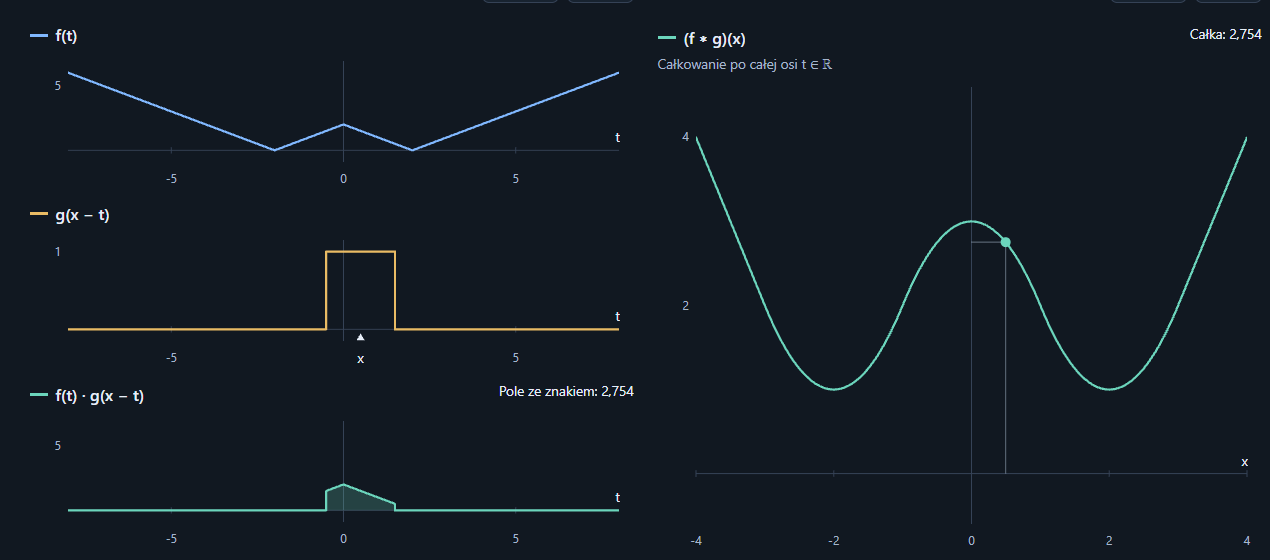
\includegraphics[width=\linewidth]{../grafika/splot-przyklad.png}
\end{center}

W naszej konstrukcji chcemy innego, bardziej przydatnego w tym kontekście
,,modyfikatora'' funkcji $f$, ale ,,wyciąganie lokalnej średniej ważonej''
to dalej główny pomysł, który stoi za tą ideą.

\begingroup
\renewcommand{\thelemat}{\arabic{lemat}a}
\begin{lemat}
\label{lem:wygladzanie-funkcji}
Niech $A\subset\R^n$ będzie zwarty, $f\colon A\to\R^n$ będzie ciągła
oraz $\varepsilon>0$. Wówczas istnieje funkcja
$g\in C^\infty(\R^n;\R^n)$ taka, że
\[
  |f(x)-g(x)|\leq\varepsilon
  \qquad\text{dla każdego }x\in A.
\]
\end{lemat}
\endgroup

\noindent\textit{Dowód.}
Do wygładzenia funkcji potrzebujemy tzw. rodziny jąder wygładzających
(z ang. \emph{mollifiers}). Połóżmy
\[
  \varphi_1(x)=
  \begin{cases}
    \displaystyle c\exp\!\left(-\frac{1}{1-|x|^2}\right), & |x|<1,\\[2mm]
    0, & |x|\geq1,
  \end{cases}
  \qquad x\in\R^n,
\]
z takim $c>0$, że
\[
  \int_{\R^n}\varphi_1(x)\,dx=1
\]
(,,wagi'' naszej ,,funkcji uśredniającej'' ,,sumują'' się do jedynki).
Naszą rodzinę definiujemy wzorem
\[
  \varphi_\alpha(x)=\alpha^{-n}\varphi_1\!\left(\frac{x}{\alpha}\right),
  \qquad x\in\R^n,\quad\alpha>0.
\]

\begin{center}
  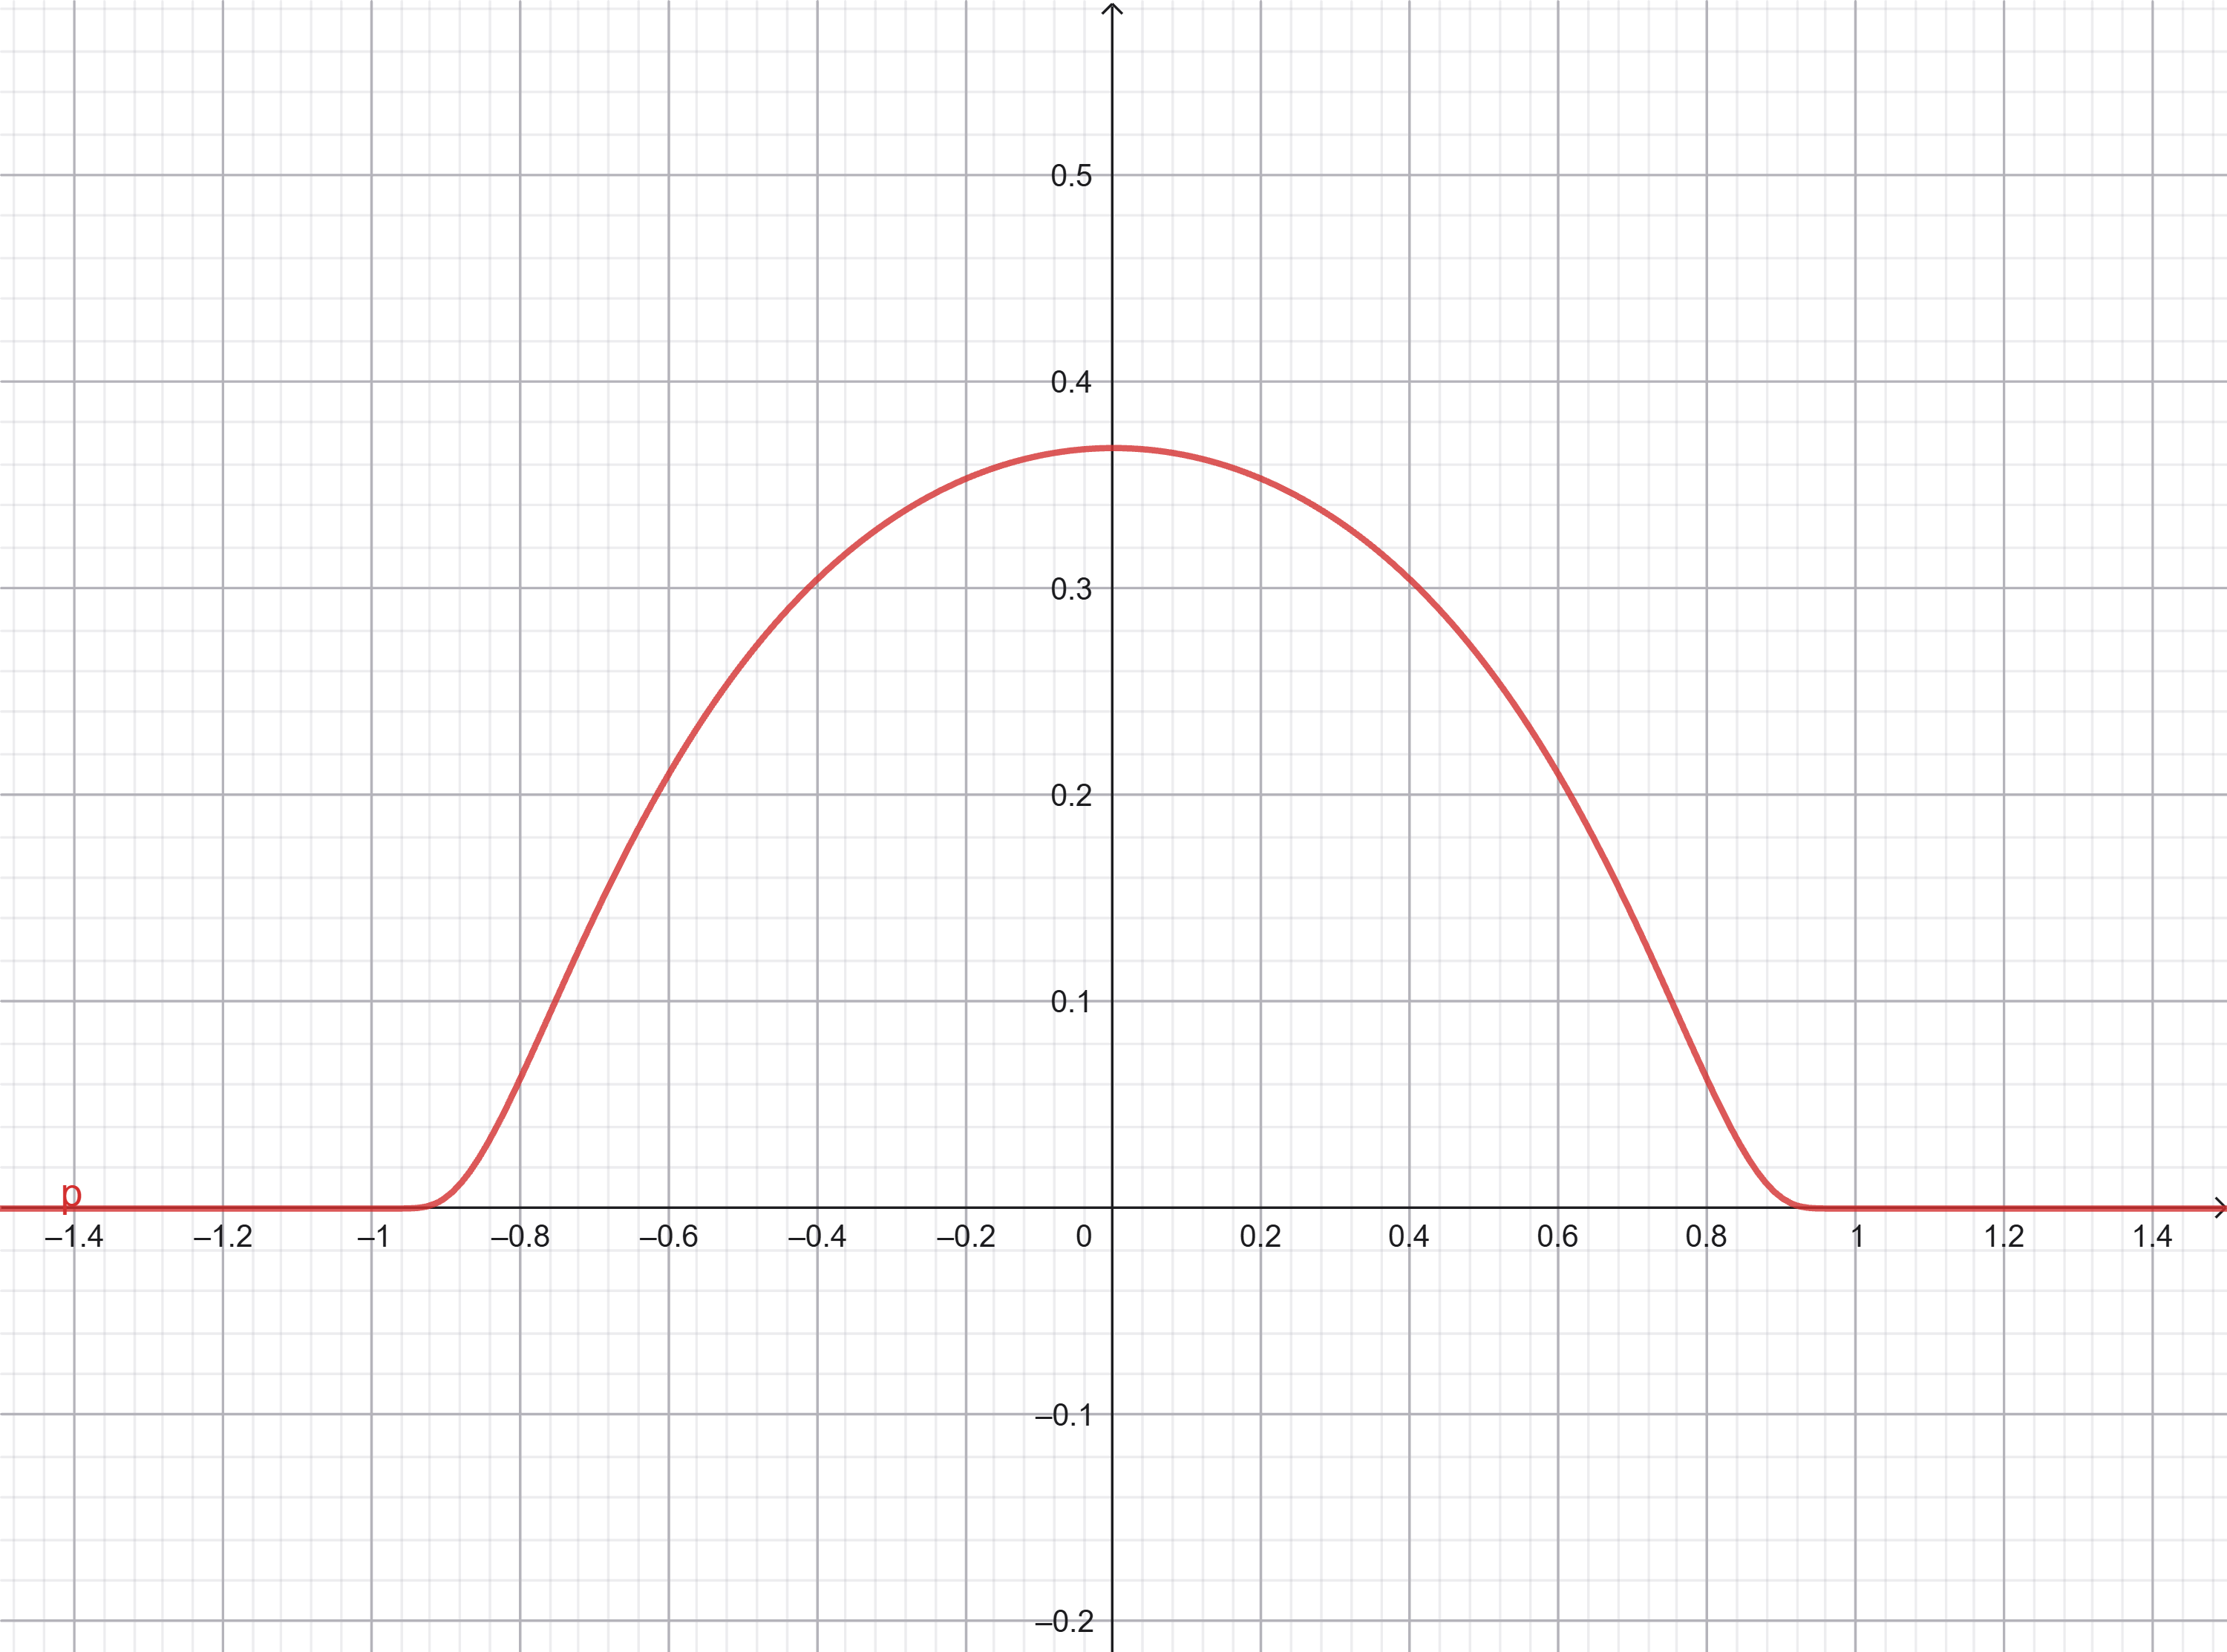
\includegraphics[width=0.84\linewidth]{../grafika/fi-1-geogebra.png}\\[0.4em]
  {\small Wykres $p(x)=\varphi_1(x)/c$ dla $n=1$, wykonany w GeoGebrze.}
\end{center}

\begin{faktbeznum}
Ustalmy $\alpha>0$. Funkcja $\varphi_\alpha\colon\R^n\to\R$ jest gładka.
\end{faktbeznum}

\begin{proof}
Funkcja $x\mapsto x/\alpha$ jest liniowa, czyli gładka. Złożenie funkcji
gładkich jest gładkie, a mnożenie przez stałą również zachowuje tę własność.
Wystarczy zatem wykazać, że $\varphi_1$ jest gładka.

\begin{samepage}
Dla $|x|<1$ mamy
\[
  1-|x|^2=1-\sum_{i=1}^n x_i^2>0.
\]
Jest to wielomian, więc funkcja gładka. Złożenie go z gładką na $(0,\infty)$
funkcją $t\mapsto1/t$, a następnie z funkcją $t\mapsto\exp(-t)$
i pomnożenie przez $c$ daje funkcję gładką.
\end{samepage}

Dla $|x|>1$ funkcja $\varphi_1$ jest stale równa $0$, więc też jest gładka.
Wystarczy zatem rozważyć punkty, w których $|x|=1$.
Połóżmy $\psi\colon\R\to\R$,
\[
  \psi(t)=
  \begin{cases}
    \exp(-1/t), & t>0,\\
    0, & t\leq0.
  \end{cases}
\]
Wówczas
\[
  \varphi_1(x)=c\,\psi\bigl(1-|x|^2\bigr),
  \qquad |x|=1\iff 1-|x|^2=0.
\]
Wystarczy więc sprawdzić gładkość $\psi$ w $0$.

Wykażemy indukcyjnie, że dla każdego $k\geq0$ istnieje wielomian $P_k$
taki, że $\psi^{(k)}$ jest ciągła oraz
\[
  \psi^{(k)}(t)=
  \begin{cases}
    P_k(1/t)e^{-1/t}, & t>0,\\
    0, & t\leq0.
  \end{cases}
\]
Dla $k=0$ bierzemy $P_0=1$. Ciągłość w $0$ wynika z granicy
$\lim_{t\to0^+}e^{-1/t}=0$.

Załóżmy, że wzór zachodzi dla $k$. Dla $t>0$, różniczkując, otrzymujemy
\[
  \psi^{(k+1)}(t)
  =\frac{1}{t^2}\bigl(P_k(1/t)-P_k'(1/t)\bigr)e^{-1/t}
  =P_{k+1}(1/t)e^{-1/t},
\]
gdzie
\[
  P_{k+1}(s)=s^2\bigl(P_k(s)-P_k'(s)\bigr).
\]
Dla $t<0$ pochodna jest równa $0$. W punkcie $0$ liczymy ją z definicji:
\[
  \lim_{t\to0^+}
  \frac{\psi^{(k)}(t)-\psi^{(k)}(0)}{t}
  =\lim_{s\to+\infty}sP_k(s)e^{-s}=0,
  \qquad s=\frac{1}{t}.
\]
Funkcja wykładnicza $e^s$ rośnie szybciej niż dowolny wielomian.
Lewostronny iloraz różnicowy jest równy $0$, więc $\psi^{(k+1)}(0)=0$.
Ponadto
\[
  \lim_{t\to0^+}\psi^{(k+1)}(t)
  =\lim_{s\to+\infty}P_{k+1}(s)e^{-s}
  =0=\psi^{(k+1)}(0),
\]
a od lewej pochodna jest stale zerowa. Zatem $\psi^{(k+1)}$ jest ciągła
w $0$, co kończy krok indukcyjny.

Otrzymujemy $\psi\in C^\infty(\R)$, a stąd gładkość $\varphi_1$
i $\varphi_\alpha$.
\end{proof}

\end{document}
